\documentclass[main.tex]{subfiles}
\begin{document}

% ── Section A: SCM Theory ───────────────────────────────────────────────────
\section{Synthetic Control \& Synthetic DiD}

% ── A0: Bridge from Blocks 1--2 ──────────────────────────────────────────
\begin{frame}{Where We Are}

  \textbf{Blocks 1 and 2 solved the multi-period, multi-cohort case:}
  \begin{itemize}\small
    \item C\&S: staggered binary absorbing treatment, many treated units
    \item dCH: non-binary, non-absorbing treatment; CGBS: continuous dose,
      staggered adoption from zero
    \item Key engine in both: \emph{many} treated units $\to$ variation
      identifies the ATT
  \end{itemize}

  \medskip
  \textbf{A case they cannot handle:}

  \begin{alertblock}{One (or very few) treated units}
    \begin{itemize}
      \item A country adopts a policy.  One region gets a shock.
        One city implements a program.
      \item With a single treated unit there are no cohorts, no
        group-time ATTs, and standard errors are not defined
        in the usual sense.
    \end{itemize}
  \end{alertblock}

  \medskip
  \textbf{This block:}
  \begin{enumerate}
    \item \textbf{Synthetic Control Method} (Abadie, Diamond \&
      Hainmueller 2010): one treated unit, build a counterfactual
      from donor pool.
    \item \textbf{Synthetic DiD} (Arkhangelsky et al.\ 2021): SCM unit
      weights + unit FE + time weights.
  \end{enumerate}

\end{frame}

% ── A1: Motivation ───────────────────────────────────────────────────────
\begin{frame}{The Single-Unit Problem}

  \textbf{Classic DiD compares treatment and control \emph{groups} under parallel
  trends.} With a single treated unit (a country, a region, a city) that
  logic strains:
  \begin{itemize}
    \item There is no treatment-group average, just one trajectory.
    \item The donor pool's \emph{average} path need not parallel the treated
      unit's pre-treatment path.
    \item Sampling-based inference is hard to justify: no well-defined
      sampling mechanism, and often the sample is the population.
  \end{itemize}

  \bigskip
  \textbf{Why not just run DiD?} DiD needs the treated--control gap to stay
  constant without treatment (parallel trends). For West Germany against the
  OECD average it already drifts before 1990 (Abadie 2021, Fig.~1A).

  \medskip
  \textbf{Synthetic control weakens it:} rather than assume a comparable control
  exists, it \emph{builds} one: a weighted combination of donor units that
  matches the treated unit's pre-treatment path.

\end{frame}

% ── A2: SCM Intuition ────────────────────────────────────────────────────
\begin{frame}{Synthetic Control: The Idea}

  \textbf{Core question:} what would the treated unit's outcome have been
  \emph{without} the intervention?

  \bigskip
  \textbf{Synthetic control answer:} find a weighted combination of donor units
  that \emph{matches the treated unit's pre-intervention trajectory}; read the
  post-intervention divergence as the effect.

  \begin{columns}[T]
    \begin{column}{0.50\textwidth}
      \textbf{Intuition:}
      \begin{itemize}
        \item No single donor looks like the treated unit.
        \item But a \emph{convex combination} of donors often can.
        \item Weights are non-negative and sum to one, an interpretable
          average with no extrapolation.
        \item Post-intervention divergence $\approx$ the effect.
      \end{itemize}
    \end{column}
    \begin{column}{0.46\textwidth}
      \begin{exampleblock}{Key advantage}
        A data-driven procedure, not an informal choice, sets the donor
        weights, and the pre-period fit is shown, not hidden as in a
        regression. The analyst still chooses the donor pool.
      \end{exampleblock}
    \end{column}
  \end{columns}

\end{frame}

% ── A3: The setting (Abadie 2021, sec. 3.1) ─────────────────────────────
\begin{frame}{The Setting}
  \small
  Abadie (2021, \textit{Journal of Economic Literature}). One unit receives
  the intervention; the others do not.

  \medskip
  \begin{tabular}{@{}lp{8.4cm}@{}}
    \toprule
    $j = 1, \dots, J+1$ & the units. Unit $1$ is the treated one; units
      $2, \dots, J+1$ are the \textbf{donor pool}: untreated, and not affected
      by the intervention. \\[2pt]
    $t = 1, \dots, T$ & the periods; the first $T_0$ come before the
      intervention. \\[2pt]
    $Y_{jt}$ & the outcome observed for unit $j$ in period $t$. \\[2pt]
    $Y^{N}_{jt}$ & the outcome unit $j$ would have had with \textbf{no}
      intervention. \\[2pt]
    $Y^{I}_{1t}$ & the outcome of the treated unit \textbf{with} the
      intervention. \\[2pt]
    $\tau_{1t} = Y^{I}_{1t} - Y^{N}_{1t}$ & the effect on the treated unit in
      period $t > T_0$: one number per period, so the effect may build up or
      fade. \\
    \bottomrule
  \end{tabular}

  \medskip
  After $T_0$ the treated unit is observed with the intervention,
  $Y_{1t} = Y^{I}_{1t}$, so the missing piece is $Y^{N}_{1t}$: what would have
  happened without it. Estimating the effect is estimating that one
  counterfactual path. Every assumption below is about $Y^{N}$; nothing is
  assumed about $Y^{I}$.
\end{frame}
% ── A3b: The synthetic control (sec. 3.2, eqs. 2–6) ─────────────────────
\begin{frame}{The Synthetic Control}
  \small
  A synthetic control is a weighted average of the donors. The weights form a
  vector $\mathbf{W} = (w_2, \dots, w_{J+1})'$ with
  \[
    w_j \ge 0, \qquad \sum_{j=2}^{J+1} w_j = 1 .
  \]
  $w_j$ is the share of the counterfactual that donor $j$ contributes; the
  shares add up to one, so the counterfactual is one whole unit assembled from
  pieces of untreated units, none subtracted. West Germany in Abadie (2021):
  0.42 Austria, 0.22 United States, 0.16 Japan, 0.11 Switzerland, 0.09
  Netherlands. Given $\mathbf{W}$, the counterfactual and the effect are
  \[
    \hat Y^{N}_{1t} = \sum_{j=2}^{J+1} w_j\, Y_{jt}, \qquad
    \hat\tau_{1t} = Y_{1t} - \hat Y^{N}_{1t}, \quad t > T_0 .
  \]
  \begin{columns}[T]
    \begin{column}{0.50\textwidth}
      \footnotesize
      \textbf{Why this form.} The comparisons everyone already makes are a
      particular $\mathbf{W}$: the plain donor average of a DiD ($w_j = 1/J$),
      a population-weighted average, or one nearest neighbour ($w_m = 1$).
      The method keeps the weighted average and lets the data set
      the weights.
    \end{column}
    \begin{column}{0.46\textwidth}
      \footnotesize
      \textbf{The two constraints.} Non-negative weights that sum to one keep
      the counterfactual inside the range of the donors: no extrapolation.
      The sum to one only makes sense if the variables are per capita
      or do not scale with size, such as prices.
    \end{column}
  \end{columns}
\end{frame}
% ── A3c: The predictors (secs. 3.1 and 3.4) ─────────────────────────────
\begin{frame}{The Predictors}
  \small
  For each unit, $k$ predictors of its outcome that the intervention does not
  affect form a vector $\mathbf{X}_j$ ($k \times 1$): covariates, often averaged
  over pre-intervention years, and pre-intervention outcome values.
  $\mathbf{X}_1$ is the treated unit's column; $\mathbf{X}_0 =
  [\mathbf{X}_2 \cdots \mathbf{X}_{J+1}]$ ($k \times J$) holds one column per
  donor. West Germany: $k = 6$, the six rows of the table, one of them the
  outcome itself, GDP per capita averaged over 1981--90.
  \medskip
  \begin{columns}[T]
    \begin{column}{0.46\textwidth}
      \footnotesize
      West Germany and the OECD average, Abadie (2021):
      \smallskip

      \begin{tabular}{@{}lrr@{}}
        \toprule
        & West Germany & OECD average \\
        \midrule
        GDP per capita & 15{,}808.9 & 13{,}669.4 \\
        trade openness & 56.8 & 59.8 \\
        inflation rate & 2.6 & 7.6 \\
        industry share & 34.5 & 33.8 \\
        schooling & 55.5 & 38.7 \\
        investment rate & 27.0 & 25.9 \\
        \bottomrule
      \end{tabular}
      \smallskip

      The plain donor average misses badly on GDP per capita, inflation and
      schooling.
    \end{column}
    \begin{column}{0.50\textwidth}
      \footnotesize
      \textbf{Two ways to fill $\mathbf{X}$.} Some covariates plus a few
      outcome years, as here; or the whole outcome path before $T_0$, in
      which case any covariates added alongside stop influencing the weights
      (Kaul, Klößner, Pfeifer and Schieler 2022). A covariate that matters and
      is left out is not asked of the synthetic unit, which may then differ on
      it.
    \end{column}
  \end{columns}
\end{frame}
% ── A4: Choosing W, the inner problem (eqs. 7–8) ────────────────────────
\begin{frame}{Choosing $\mathbf{W}$: the Inner Problem}
  \small
  In practice the user supplies the predictors and the pre-intervention years,
  and the software returns $\mathbf{W}^{*}$. What it minimises:
  \[
    \sum_{h=1}^{k} v_h \Big( X_{h1} - \sum_{j=2}^{J+1} w_j X_{hj} \Big)^2
    \qquad \text{subject to } w_j \ge 0,\ \sum_j w_j = 1 .
  \]
  Term by term: for predictor $h$, the gap between the treated unit's value
  $X_{h1}$ and the synthetic unit's $\sum_j w_j X_{hj}$, squared, times its
  importance $v_h$. $\mathbf{W}^{*}$ makes the sum of the $k$ weighted gaps as
  small as possible, with non-negative weights that sum to one: the synthetic
  unit that resembles the treated unit most on the predictors, counting the
  important ones more. The $v_h$ can be fixed by a rule (inverse variance) or
  chosen from the data in a second, outer problem.
  \smallskip
  \begin{columns}[T]
    \begin{column}{0.50\textwidth}
      \footnotesize
      \begin{tabular}{@{}lrr@{}}
        \toprule
        Predictor & West Germany & synthetic \\
        \midrule
        GDP per capita & 15{,}808.9 & 15{,}802.2 \\
        trade openness & 56.8 & 56.9 \\
        inflation rate & 2.6 & \alert{3.5} \\
        industry share & 34.5 & 34.4 \\
        schooling & 55.5 & 55.2 \\
        investment rate & 27.0 & 27.0 \\
        \bottomrule
      \end{tabular}
    \end{column}
    \begin{column}{0.46\textwidth}
      \footnotesize
      Five of six predictors reproduced. Inflation is the exception: West
      Germany's $2.6$ was too low for the synthetic unit to reproduce
      (fn.~16). The gaps $\mathbf{X}_1 - \mathbf{X}_0 \mathbf{W}^{*}$ must be
      checked and reported.
    \end{column}
  \end{columns}
\end{frame}
% ── A4b: Choosing V, the outer problem (pp. 396–397) ─────────────────────
\begin{frame}{Choosing $\mathbf{V}$: the Outer Problem}
  \small
  $v_h$ should measure how much predictor $h$ helps to predict the outcome
  without intervention after $T_0$. That outcome is never observed, but before
  $T_0$ it is, so the software calibrates the importances on the years before
  the intervention: it tries importance vectors $\mathbf{V}$; for each one it
  computes $\mathbf{W}(\mathbf{V})$ as on the previous frame; it measures how
  closely that synthetic unit follows the treated outcome before $T_0$; and it
  keeps the $\mathbf{V}$ that follows it best:
  \[
    \mathbf{V}^{*} = \arg\min_{\mathbf{V}} \sum_{t \le T_0}
    \Big( Y_{1t} - \sum_{j=2}^{J+1} w_j(\mathbf{V})\, Y_{jt} \Big)^2,
  \]
  the sum, over the years before $T_0$, of the synthetic unit's squared error.
  In words: the outcome before the intervention decides how much each
  predictor counts, $\mathbf{V}$; matching the predictors with those counts
  decides how much each donor counts, $\mathbf{W}$.
  \medskip
  \begin{columns}[T]
    \begin{column}{0.52\textwidth}
      \footnotesize
      \textbf{What the user decides.} Which predictors enter, which outcome
      years, and over which pre-intervention years the fit is measured. The
      search itself comes built in, in a quick approximate version and in a
      full, slower one. An alternative chooses $\mathbf{V}$ out of sample,
      on a training and a later validation stretch of the pre-period.
    \end{column}
    \begin{column}{0.44\textwidth}
      \footnotesize
      \textbf{Not unique.} The $\mathbf{V}$ chosen out of sample may not be
      unique (fn.~7); the paper asks to show that the results are not overly
      sensitive to the choice of $\mathbf{V}$.
    \end{column}
  \end{columns}
\end{frame}
% ── A4c: What the fit tells you (Figure 1, pp. 397–403) ──────────────────
\begin{frame}{What the Fit Tells You}
  \small
  Two checks follow the estimation, and both are visible in the data.
  \begin{enumerate}\small
    \item \textbf{The predictors:} $\mathbf{X}_1 \approx \mathbf{X}_0
      \mathbf{W}^{*}$, predictor by predictor: the balance table of
      ``Choosing $\mathbf{W}$''.
    \item \textbf{The outcome before $T_0$:} the synthetic unit should follow
      $Y_{1t}$ over the whole pre-intervention period. In West Germany the
      plain OECD average drifts away from GDP per capita for decades before
      1990; the synthetic unit tracks it until 1990. One number summarises
      this fit: the root mean squared prediction error
      before $T_0$, the typical distance between $Y_{1t}$ and $\hat Y^{N}_{1t}$
      in the outcome's units; the placebo test divides by it.
  \end{enumerate}
  \medskip
  What the method exploits is the co-movement of the outcome across units:
  GDP per capita moves together across countries, so a weighted
  average of a few of them can follow one of them for thirty years.
  \medskip
  \begin{block}{\footnotesize Post-intervention outcomes never enter}
    \footnotesize The weights depend on pre-intervention data only. They can
    be computed, and registered, before the post-intervention outcomes exist.
  \end{block}
\end{frame}
% ── A5: Inference by permutation (Abadie 2021, sec. 3.5) ─────────────────
\begin{frame}{Inference: the In-Space Placebo}
  \small
  \textbf{In a nutshell.} Give the intervention, on paper, to each donor in
  turn and estimate its ``effect'' with the same method. Nothing happened to
  the donors, so those effects are what the method produces by chance. The
  treated unit's effect is evidence when it is larger than all, or almost all,
  of them.
  \medskip

  \textbf{The $p$-value.} The share of the $J+1$ units whose effect is at least
  as large as the treated unit's. If the treated unit ranks first,
  $p = 1/(J+1)$, and no smaller value exists: with $20$ donors, $p$ never goes
  below $1/21$.
  \medskip

  \textbf{How ``large'' is measured.} By the gap after $T_0$ relative to the
  fit before $T_0$, both as root mean squared gaps, so that a donor the method
  never fitted well does not pass for an effect:
  \[
    r_j = \frac{\text{root mean squared gap after } T_0}
               {\text{root mean squared gap before } T_0}.
  \]
\end{frame}
% ── A5b: In-space placebo, the cutoff and the three p's per year ─────────
\begin{frame}{In-Space Placebo: the Cutoff and the Three $p$-Values per Year}
  \small
  \textbf{The cutoff.} A donor whose synthetic control fits badly before
  $T_0$ has large gaps in every year, before and after, and looks
  ``extreme'' without any effect. Donors whose pre-period mean squared gap is more than
  $k$ times the treated unit's are dropped before the year-by-year
  $p$-values; with $m$ units left, the smallest $p$ is $1/m$.
  \medskip

  \textbf{Three $p$-values per year.} For each year after $T_0$, the treated
  unit's gap is compared with the placebo gaps of that same year, the treated
  unit counting itself:
  \begin{itemize}\small
    \item \textbf{left-sided:} the share of gaps at least as negative as the
      treated unit's;
    \item \textbf{right-sided:} the share at least as positive;
    \item \textbf{two-sided:} the share at least as large in absolute value,
      in either direction.
  \end{itemize}
  \medskip
  Six units, treated gap $-10$, placebo gaps $-12$, $-3$, $0$, $+4$, $+11$:
  left-sided $2/6$ ($-12$ and the treated unit), right-sided $5/6$ (all but
  $-12$), two-sided $3/6$ ($-12$, $+11$ and the treated unit).
\end{frame}
% ── A5c: Robustness: in-time placebo (sec. 7, p. 414) ────────────────────
\begin{frame}{Robustness: the In-Time Placebo}
  \small
  Move the intervention back to a year $T_0' < T_0$ when nothing happened,
  drop every predictor measured after $T_0'$, and re-estimate as if the
  intervention had come then.
  \medskip
  \begin{columns}[T]
    \begin{column}{0.52\textwidth}
      \centering
      \begin{tikzpicture}[x=1cm, y=1cm, font=\scriptsize]
        \draw[->] (0,0) -- (6.4,0) node[right] {$t$};
        \draw[->] (0,-2.2) -- (0,1.3) node[above] {gap};
        \draw[dotted] (0,0) -- (6.2,0);
        \draw[dashed, gray] (2.0,-2.1) -- (2.0,0.9) node[above] {$T_0'$};
        \draw[dashed, gray] (4.4,-2.1) -- (4.4,0.9) node[above] {$T_0$};
        \draw[thick, MidBlue] (0.2,0.1) -- (0.8,-0.1) -- (1.4,0.15) -- (2.0,-0.05)
          -- (2.6,0.1) -- (3.2,-0.1) -- (3.8,0.1) -- (4.4,0) -- (4.8,-0.6)
          -- (5.2,-1.1) -- (5.6,-1.5) -- (6.0,-1.8);
        \draw[<->, AlertRed] (2.05,-0.9) -- (4.35,-0.9)
          node[midway, below, AlertRed] {stay near 0};
      \end{tikzpicture}
    \end{column}
    \begin{column}{0.44\textwidth}
      \footnotesize
      Between $T_0'$ and $T_0$ the gap should stay near zero: the synthetic
      unit keeps following the treated unit when nothing happens to it.
      \medskip

      A gap that opens before $T_0$ is a drift of the method itself. The
      effect after $T_0$ then has to be much larger than that drift to
      count.
    \end{column}
  \end{columns}
\end{frame}
% ── A5d: Robustness: leave-one-out and predictors (sec. 7, p. 415) ───────
\begin{frame}{Robustness: Leave-One-Out and the Predictor Set}
  \small
  \textbf{Leave-one-out.} Drop each donor with positive weight, one at a time,
  and re-estimate. Trajectories that stay close to the original say the
  result rests on no single donor; one that jumps names the donor it rests on.
  Abadie (2021, Fig.~4) plots every trajectory beside the original; here we
  also report the range of the gap.
  \medskip

  \textbf{The predictor set.} Another set of predictors gives another
  $\mathbf{W}^{*}$, another fit before $T_0$ and another gap. To choose the
  set, fit the weights on the earlier pre-years and keep the set that best
  predicts the later ones (p.~402). Show the alternatives beside it; the
  conclusion should hold across them (p.~415).
\end{frame}
% ── A6: Requirements (secs. 5–7) ─────────────────────────────────────────
\begin{frame}{Requirements: Context and Data}
  \footnotesize
  \begin{columns}[T]
    \begin{column}{0.52\textwidth}
      \textbf{Context}
      \begin{itemize}\footnotesize
        \item \textbf{Effect against volatility.} A small effect is lost in
          the treated unit's own shocks; common shocks are differenced out,
          unit-specific ones are not.
        \item \textbf{A comparison group exists.} Drop donors with similar
          interventions or large idiosyncratic shocks; the rest should
          resemble the treated unit.
        \item \textbf{No anticipation.} If agents react early, move the
          intervention date back in the data.
        \item \textbf{No interference.} Drop exposed donors; same-sign
          spillovers left in attenuate the estimate.
        \item \textbf{Within reach of the donors.} Level out of reach and
          only the trend matters: differences, growth rates, demeaning or an
          intercept (synthetic DiD).
        \item \textbf{Time horizon.} Effects that build up need post-periods.
      \end{itemize}
    \end{column}
    \begin{column}{0.44\textwidth}
      \textbf{Data}
      \begin{itemize}\footnotesize
        \item Aggregate series for predictors and outcomes, official or built
          from microdata.
        \item A long pre-intervention window: a short one invites a fit that
          is spurious. If the window is long enough to
          hold structural breaks, weight recent predictors more through
          $\mathbf{V}$.
        \item Enough post-intervention periods for the effect to appear.
      \end{itemize}
    \end{column}
  \end{columns}
\end{frame}
% ── A7: SCM in the wild (bridge theory -> demo) ──────────────────────────
\begin{frame}{Synthetic Control: Published Applications}

  \textbf{The same recipe, one treated unit, a long pre-period and a credible
  donor pool, in five published cases:}

  \medskip
  \begin{itemize}\small
    \item \textbf{Abadie \& Gardeazabal (2003)}: the economic cost of terrorism
      in the Basque Country (the original SCM).
    \item \textbf{Abadie, Diamond \& Hainmueller (2010)}: California's
      Proposition 99 tobacco tax \emph{(our demo)}.
    \item \textbf{Abadie, Diamond \& Hainmueller (2015)}: German reunification
      and per-capita GDP.
    \item \textbf{Born et al.\ (2019)}: the Brexit vote and UK output.
    \item \textbf{Grier \& Maynard (2016)}: the economic consequences of
      Hugo Ch\'avez.
  \end{itemize}

  \medskip
  Conflict, macro, trade, politics: the same method. The demo works the
  second case.

\end{frame}

% ── Section B: Demo — California Prop 99 (SCM via synth2) ──────────────
\section{Demo: California Prop 99 --- SCM}

% ── B1: Context & Data ───────────────────────────────────────────────────
\begin{frame}{Case --- California Prop 99: Context \& Data}

  \begin{columns}[T]
    \begin{column}{0.54\textwidth}
      \textbf{Research question}\\
      Did Proposition 99 (in force January 1989; cigarette tax raised by
      \$0.25/pack) cut per-capita tobacco consumption?

      \medskip
      \textbf{Paper / data}\\
      Abadie, Diamond \& Hainmueller (2010), \textit{JASA};
      \texttt{smoking.dta}.
      \begin{itemize}\small
        \item Panel: \textbf{39 US states}, 1970--2000.
        \item Treated: \textbf{California} (\texttt{state==3});
          donor pool: 38 states.
        \item Outcome \texttt{cigsale} (packs p.c.); predictors: log GDP p.c.,
          beer, share aged 15--24, retail price, lagged \texttt{cigsale}.
      \end{itemize}
    \end{column}
    \begin{column}{0.42\textwidth}
      \begin{block}{Why SCM here?}
        \footnotesize
        One treated unit $\Rightarrow$ C\&S / dCH do not apply. No single
        state matches California's pre-1989 path, but a convex combination
        of donors can.
      \end{block}
      \medskip
      \footnotesize We implement it with \texttt{synth2} (Yan \& Chen 2023),
      which wraps \texttt{synth} and automates placebo tests, the
      leave-one-out check, and the figures.
    \end{column}
  \end{columns}

\end{frame}

% ── B2: synth2 command ───────────────────────────────────────────────────
\begin{frame}[fragile]{Stata: the \texttt{synth2} Command}

\begin{lstlisting}[language=,basicstyle=\ttfamily\footnotesize,
    keywordstyle=\color{MidBlue}\bfseries, commentstyle=\color{gray},
    morekeywords={synth2,xtset}, xleftmargin=2mm]
use "$data/smoking.dta", clear
xtset state year                       // state 3 = California

synth2 cigsale lnincome age15to24 retprice beer ///
    cigsale(1988) cigsale(1980) cigsale(1975),  ///  predictors + lagged outcomes
    trunit(3) trperiod(1989)                    ///  treated unit & date
    xperiod(1980(1)1988) nested allopt              // ADH spec
\end{lstlisting}

  \footnotesize
  \begin{itemize}\footnotesize
    \item \texttt{trunit(3) trperiod(1989)}: California, treated from 1989.
    \item \texttt{xperiod(1980(1)1988)}: average the predictors without their own
      year over 1980--1988.
    \item \texttt{nested allopt}: the full search for $\mathbf{V}$. Every block
      keeps it except the in-space placebo, where 39 full searches would take
      over an hour.
    \item Add \texttt{placebo(unit cutoff(2))}, \texttt{placebo(period(1985))},
      or \texttt{loo} for inference and robustness (next slides).
  \end{itemize}

\end{frame}

% ── B3: Output — weights + fit ───────────────────────────────────────────
\begin{frame}{Output: Synthetic California}

  \begin{columns}[T]
    \begin{column}{0.40\textwidth}
      \textbf{Optimal unit weights,} the $\mathbf{W}^{*}$ of ``Choosing
      $\mathbf{W}$'':
      \smallskip
      \footnotesize
      \begin{tabular}{lc}
        \toprule
        State & Weight \\
        \midrule
        Utah        & 33.5\% \\
        Nevada      & 23.5\% \\
        Montana     & 20.2\% \\
        Colorado    & 16.0\% \\
        Connecticut & 6.8\% \\
        \bottomrule
      \end{tabular}

      \medskip
      \normalsize
      All other 33 donors get weight 0: with California outside the donors'
      convex hull, at most as many donors as predictors (7) carry weight
      (Abadie 2021).
    \end{column}
    \begin{column}{0.56\textwidth}
      \textbf{Pre-treatment fit:}
      \begin{itemize}
        \item \textbf{RMSPE} $= 1.75$, \quad $R^2 = 0.97$.
        \item Predictor balance is tight: synthetic California matches the
          treated unit far better than the simple donor average (e.g.\
          \texttt{cigsale(1988)} bias $1.7\%$ vs $26\%$).
        \item Predictor importance ($\mathbf{V}$) concentrates on
          \texttt{age15to24}, \texttt{cigsale(1975)} and \texttt{retprice}
          (next frame).
      \end{itemize}

      \medskip
      \footnotesize Same five donors as Abadie et al.\ (2010, Table 2);
      \texttt{synth2}'s weights differ from theirs by at most 0.4 points.
    \end{column}
  \end{columns}

\end{frame}

% ── B3a: Output — balance plot and V bars ────────────────────────────────
\begin{frame}{Output: Balance and Predictor Importance}
  \begin{columns}[T]
    \begin{column}{0.50\textwidth}
      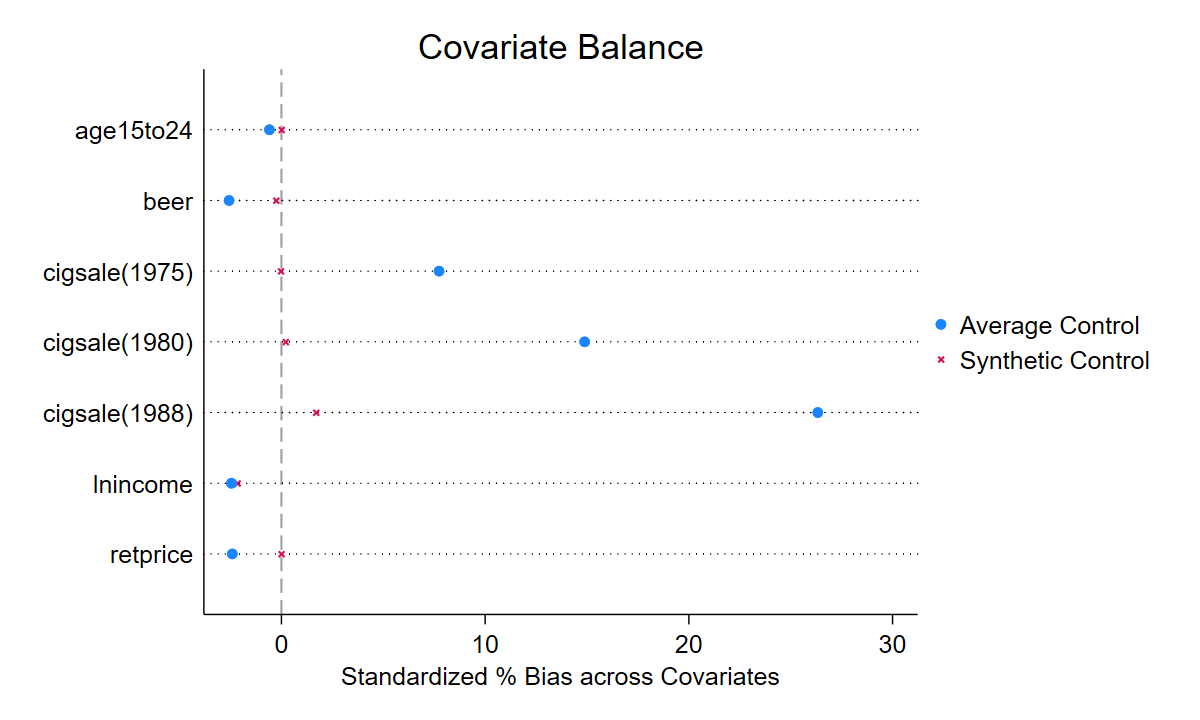
\includegraphics[width=\linewidth]{figures/scm/scm_bias.png}
    \end{column}
    \begin{column}{0.50\textwidth}
      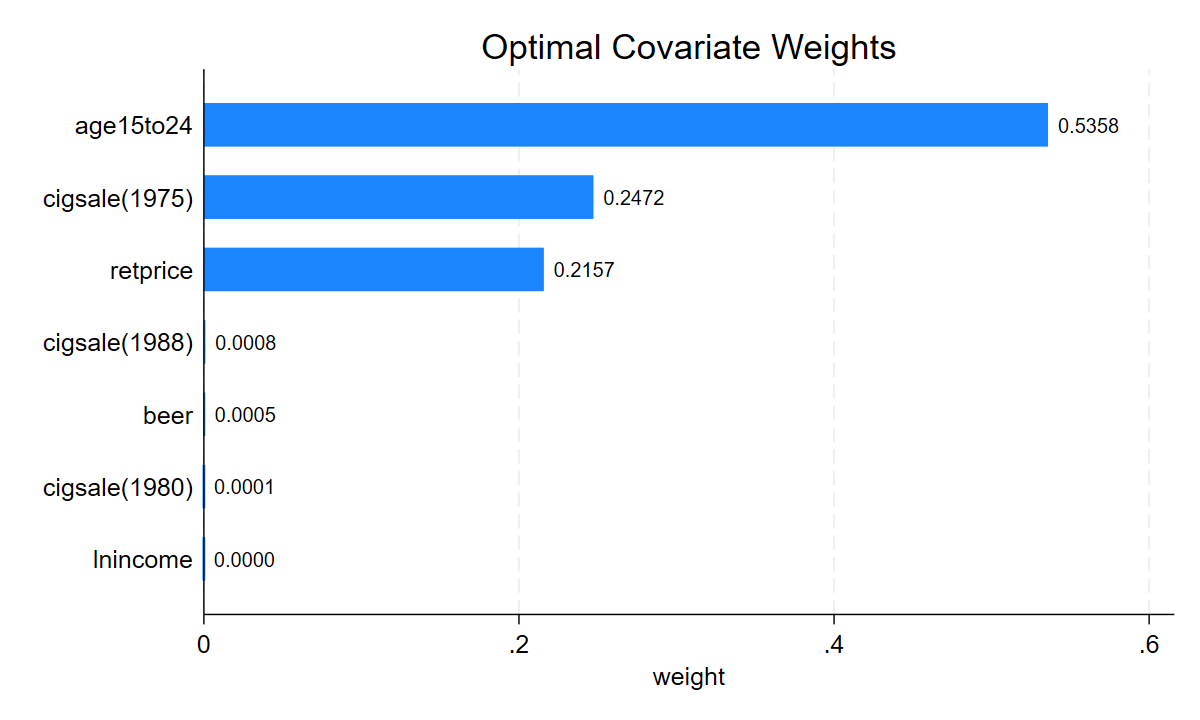
\includegraphics[width=\linewidth]{figures/scm/scm_weight_vars.png}
    \end{column}
  \end{columns}
  \vspace{-1mm}
  \footnotesize
  \textbf{Left:} predictor balance, the gaps $\mathbf{X}_1 - \mathbf{X}_0
  \mathbf{W}^{*}$ of the theory as a plot. For each predictor, how far
  California is from the synthetic unit built with $\mathbf{W}^{*}$ (crosses)
  and from the plain donor average (dots), in per cent of California's
  value. The synthetic unit is within $2.2\,\%$ on every predictor; the plain average is $26\,\%$
  off on 1988 sales and $15\,\%$ on 1980 sales.
  \textbf{Right:} the importance $v_h$ the search gave each predictor
  (``Choosing $\mathbf{V}$''). Three carry all of it: \texttt{age15to24}
  $0.54$, \texttt{cigsale(1975)} $0.25$, \texttt{retprice} $0.22$. Other
  searches return other $\mathbf{V}$ and other weights: the quick search of
  the placebos gives RMSPE $2.04$ and ATT $-18.0$ (here $1.75$, $-19.0$).
\end{frame}

% ── B4: Figure — path ────────────────────────────────────────────────────
\begin{frame}{California vs Synthetic California}

  \begin{center}
    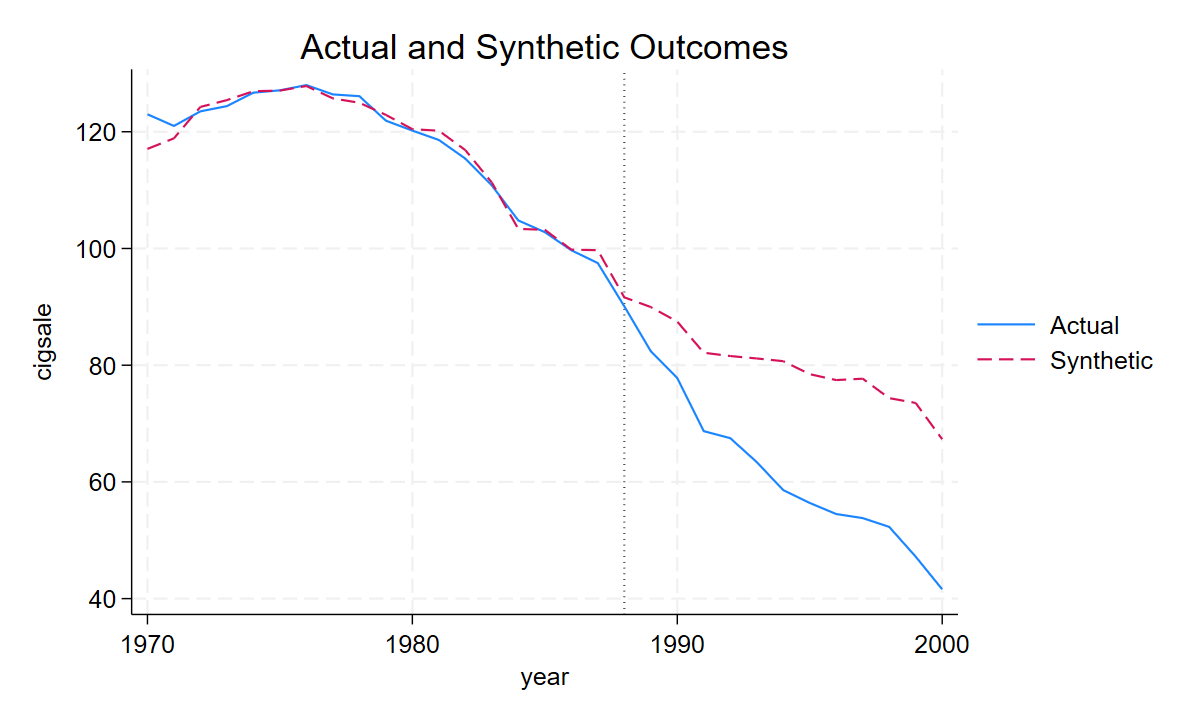
\includegraphics[width=0.70\textwidth]{figures/scm/scm_path.png}
  \end{center}

  \vspace{-3mm}
  \small
  \textbf{Reading it:} the second check of ``What the Fit Tells You'': the
  two series track closely before 1989 (RMSPE $1.75$ packs). After Prop 99,
  California diverges downward.

\end{frame}

% ── B5: Figure — treatment effects (gap) ─────────────────────────────────
\begin{frame}{The Effect Over Time}

  \begin{center}
    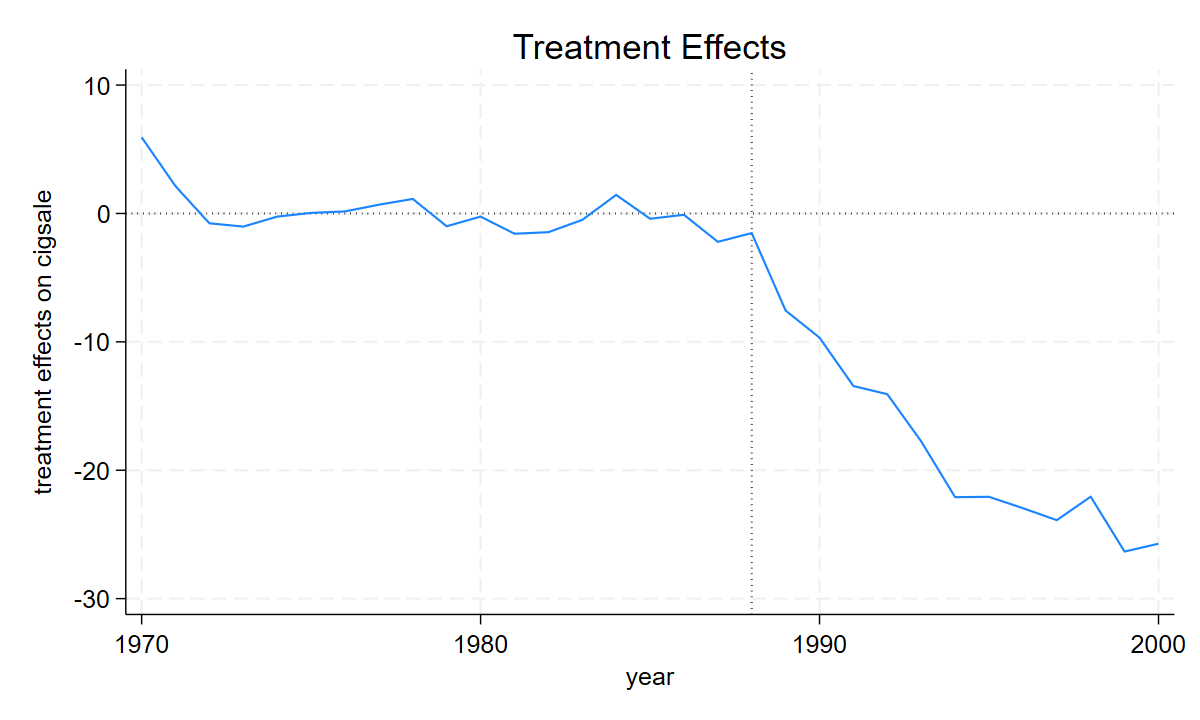
\includegraphics[width=0.70\textwidth]{figures/scm/scm_effects.png}
  \end{center}

  \vspace{-3mm}
  \small
  \textbf{Reading it:} the effect $\hat\tau_{1t}$ of ``The Synthetic
  Control'', year by year. The gap is
  $\approx 0$ pre-1989, then grows to $\approx -26$ packs by 2000. Average
  post-treatment effect (ATT) $= \mathbf{-19.0}$ packs per capita.

\end{frame}

% ── B6: Figure — in-space placebo ────────────────────────────────────────
\begin{frame}{Inference: In-Space Placebo Test}

  \begin{columns}[T]
    \begin{column}{0.62\textwidth}
      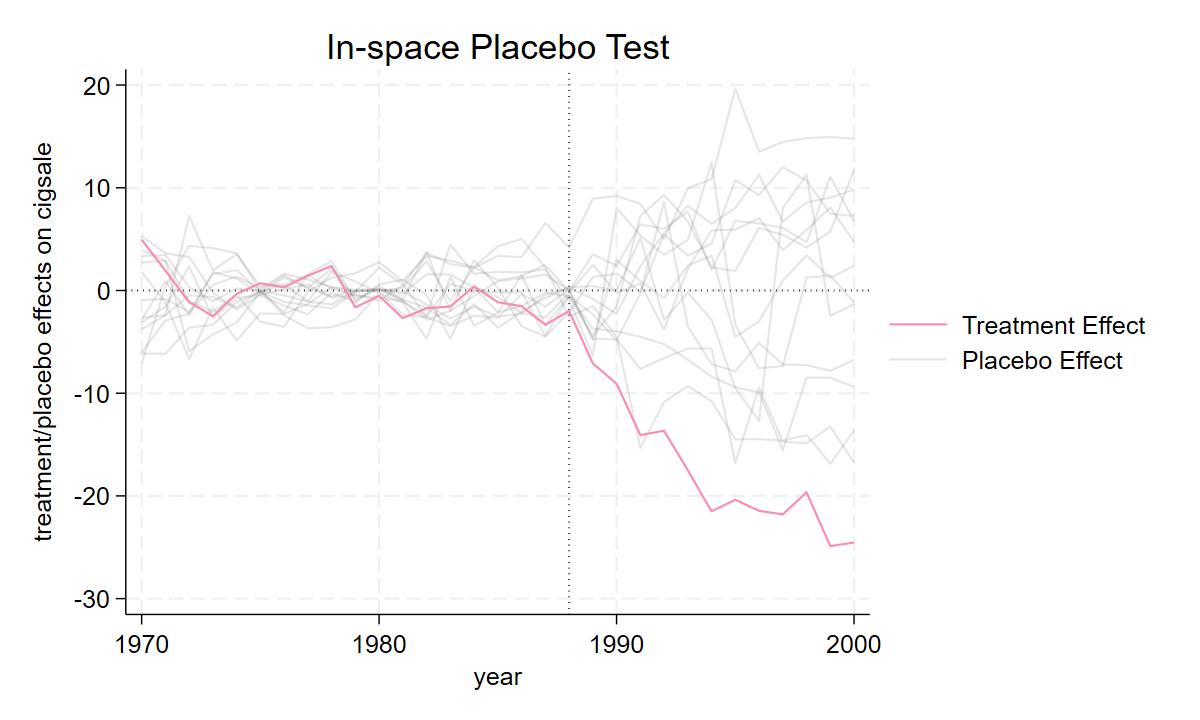
\includegraphics[width=\linewidth]{figures/scm/scm_placebo.png}
    \end{column}
    \begin{column}{0.36\textwidth}
      \footnotesize
      Each of the 39 units gets its own synthetic control; the figure shows
      California (pink) and the 13 donors kept by \texttt{cutoff(2)}.
      California's gap is the most extreme from 1992 on. This block
      runs the quick search, so California's own fit here is RMSPE $2.04$
      rather than $1.75$.\\[4pt]
      \textbf{One number per unit:} the mean squared gap after 1989 divided
      by the mean squared gap before, the ratio the command prints (taking
      roots would not change the ranking). California $85$; Georgia comes
      next with $64$; 29 of the 38 donors are below $10$.\\[4pt]
      \textbf{The $p$-value:} California ranks first of 39, so
      $p = 1/39 = 0.026$, the floor.
    \end{column}
  \end{columns}

\end{frame}

% ── B6b: Figure — MSPE ratios ranked, and the cutoff table ──────────────
\begin{frame}{In-Space Placebo: the Ranking and the Cutoff}
  \begin{columns}[T]
    \begin{column}{0.44\textwidth}
      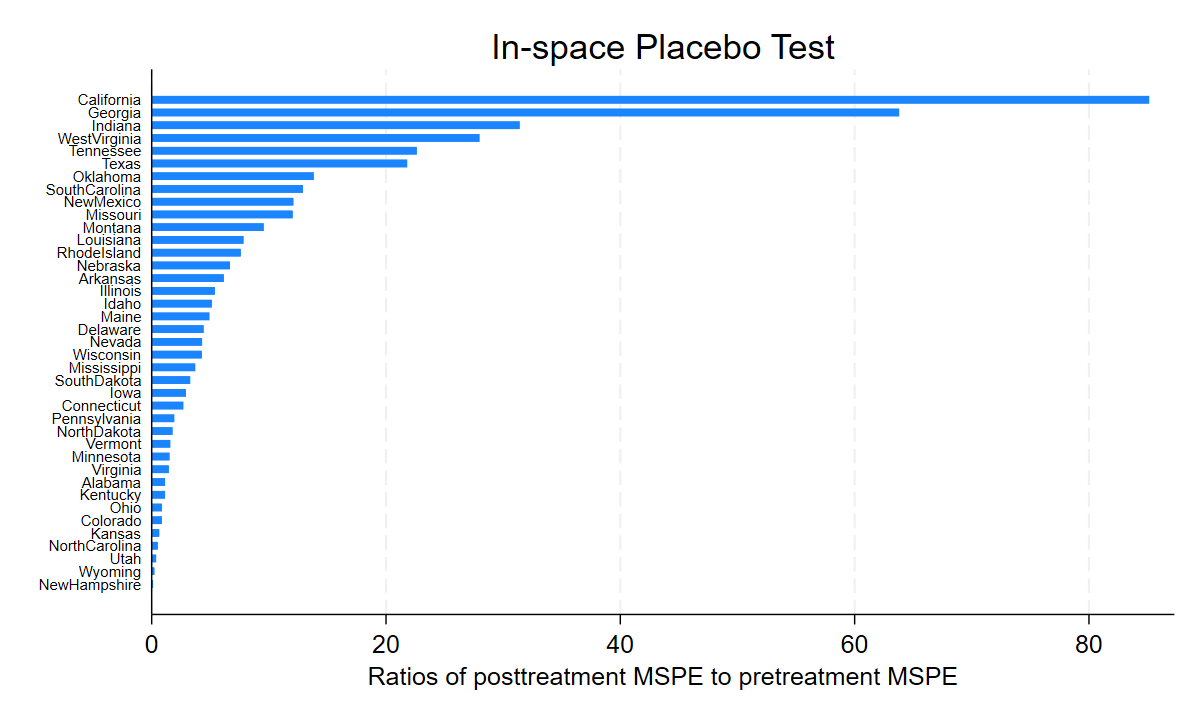
\includegraphics[width=\linewidth]{figures/scm/scm_mspe_ratio.png}

      \footnotesize
      The 39 ratios ranked, one bar per unit: California $85$, Georgia $64$,
      Indiana $31$, then a long tail. First of 39: $p = 1/39$.
    \end{column}
    \begin{column}{0.54\textwidth}
      \footnotesize
      Rows of the table the command prints (mean squared gaps):
      \smallskip

      {\scriptsize\setlength{\tabcolsep}{3.5pt}
      \begin{tabular}{@{}lrrrrl@{}}
        \toprule
        unit & pre & post & ratio & pre / pre CA & \texttt{cutoff(2)} \\
        \midrule
        California & 4.2 & 353.6 & 85.1 & 1.0 & \\
        Georgia & 1.9 & 122.8 & 63.8 & 0.5 & kept \\
        Indiana & 40.6 & 1276.1 & 31.4 & 9.8 & out \\
        Nevada & 59.6 & 256.1 & 4.3 & 14.3 & out \\
        Colorado & 36.5 & 31.8 & 0.9 & 8.8 & out \\
        Connecticut & 27.2 & 73.4 & 2.7 & 6.6 & out \\
        Utah & 593.8 & 223.3 & 0.4 & 143.0 & out \\
        Kentucky & 683.5 & 778.8 & 1.1 & 164.6 & out \\
        New Hampshire & 3485.5 & 312.8 & 0.1 & 839.3 & out \\
        \bottomrule
      \end{tabular}}
      \smallskip

      \textbf{The cutoff:} a donor stays if its pre-1989 error is at most
      twice California's, last column $\le 2$. 13 of the 38 donors stay; with
      California, 14 units. Utah, Nevada, Colorado and Connecticut, four of
      California's five donors, have no good synthetic control of their own
      and go; Montana stays. California still ranks first among the 14:
      $p = 1/14 = 0.071$, the floor for every year-by-year $p$.
    \end{column}
  \end{columns}
\end{frame}

% ── B6c: Table — the three p-values per year ────────────────────────────
\begin{frame}{In-Space Placebo: Three $p$-Values per Year}
  \begin{columns}[T]
    \begin{column}{0.44\textwidth}
      \footnotesize
      The table the command prints, among the 14 units kept:
      \smallskip

      {\scriptsize
      \begin{tabular}{@{}lrrrr@{}}
        \toprule
        year & gap & two-sided & right & left \\
        \midrule
        1989 & $-7.1$ & 0.143 & 1.000 & 0.071 \\
        1990 & $-9.1$ & 0.143 & 1.000 & 0.071 \\
        1991 & $-14.1$ & 0.143 & 0.929 & 0.143 \\
        1992 & $-13.7$ & 0.071 & 1.000 & 0.071 \\
        1993 & $-17.5$ & 0.071 & 1.000 & 0.071 \\
        1994 & $-21.5$ & 0.071 & 1.000 & 0.071 \\
        1995 & $-20.4$ & 0.071 & 1.000 & 0.071 \\
        1996 & $-21.5$ & 0.071 & 1.000 & 0.071 \\
        1997 & $-21.8$ & 0.071 & 1.000 & 0.071 \\
        1998 & $-19.6$ & 0.071 & 1.000 & 0.071 \\
        1999 & $-24.9$ & 0.071 & 1.000 & 0.071 \\
        2000 & $-24.5$ & 0.071 & 1.000 & 0.071 \\
        \bottomrule
      \end{tabular}}
    \end{column}
    \begin{column}{0.54\textwidth}
      \footnotesize
      Each year, California's gap against the 13 placebo gaps of that year,
      California counting itself: $0.071 = 1/14$, $0.143 = 2/14$.
      \begin{itemize}\footnotesize
        \item \textbf{Left}, gaps at least as negative as California's:
          $1/14$ every year but 1991, when one donor fell more. The one to
          read: Prop 99 was meant to cut sales.
        \item \textbf{Right}, gaps at least as positive: $14/14$ every year
          but 1991. California's gap is the lowest, so every placebo gap lies
          above it.
        \item \textbf{Two-sided}, gaps at least as large in either direction:
          $2/14$ in 1989--1991, $1/14$ from 1992. In 1989--90 one donor had a
          positive gap as large as California's negative one.
      \end{itemize}
      The three plots the command draws are these three columns against the
      year.
    \end{column}
  \end{columns}
\end{frame}

% ── B7: Figure — in-time placebo ─────────────────────────────────────────
\begin{frame}{Robustness: In-Time Placebo (fake 1985)}

  \begin{center}
    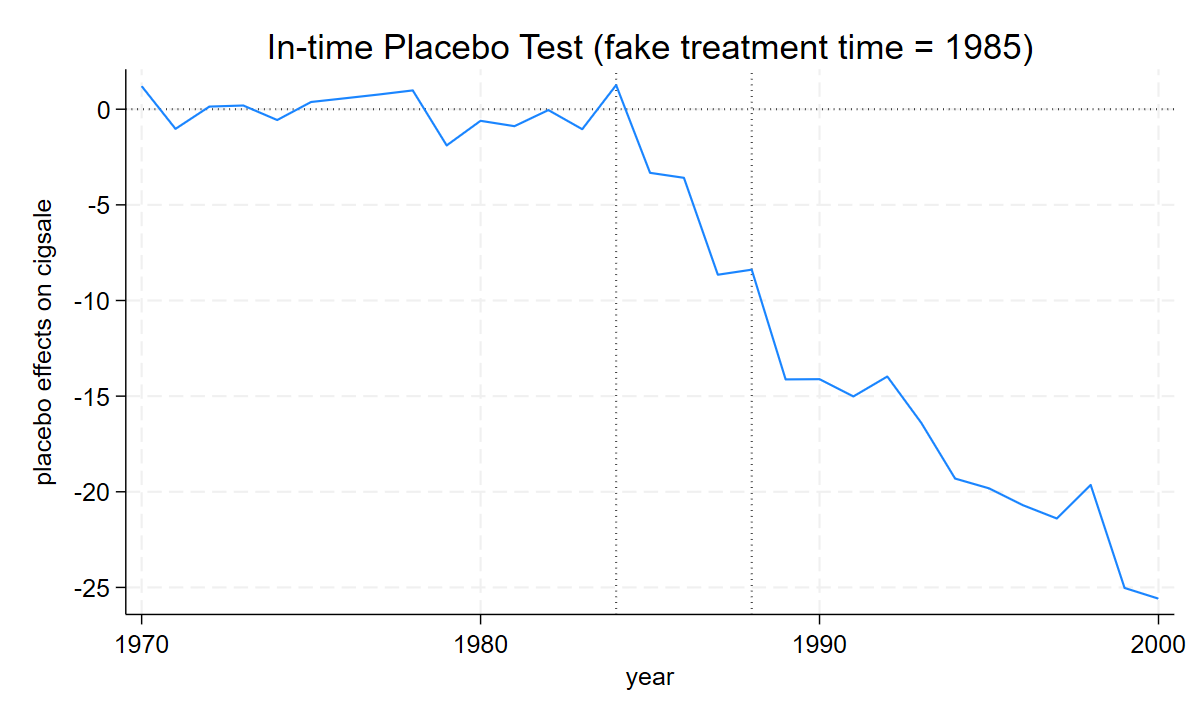
\includegraphics[width=0.66\textwidth]{figures/scm/scm_intime.png}
  \end{center}

  \vspace{-3mm}
  \small
  \textbf{Reading it:} the check of ``Robustness: the In-Time Placebo''.
  With the treatment moved to 1985 the gap
  stays small in 1985--86 ($\approx -3$), but it already reaches $\approx -8$
  by 1987--88, a mild pre-existing drift. The \emph{much} larger divergence
  (to $-25$) still comes after 1989, so the effect is not purely a pre-trend;
  but read this as a \emph{weaker} check than the in-space test.

\end{frame}

% ── B8: Figure — leave-one-out ───────────────────────────────────────────
\begin{frame}{Robustness: Leave-One-Out}

  \begin{center}
    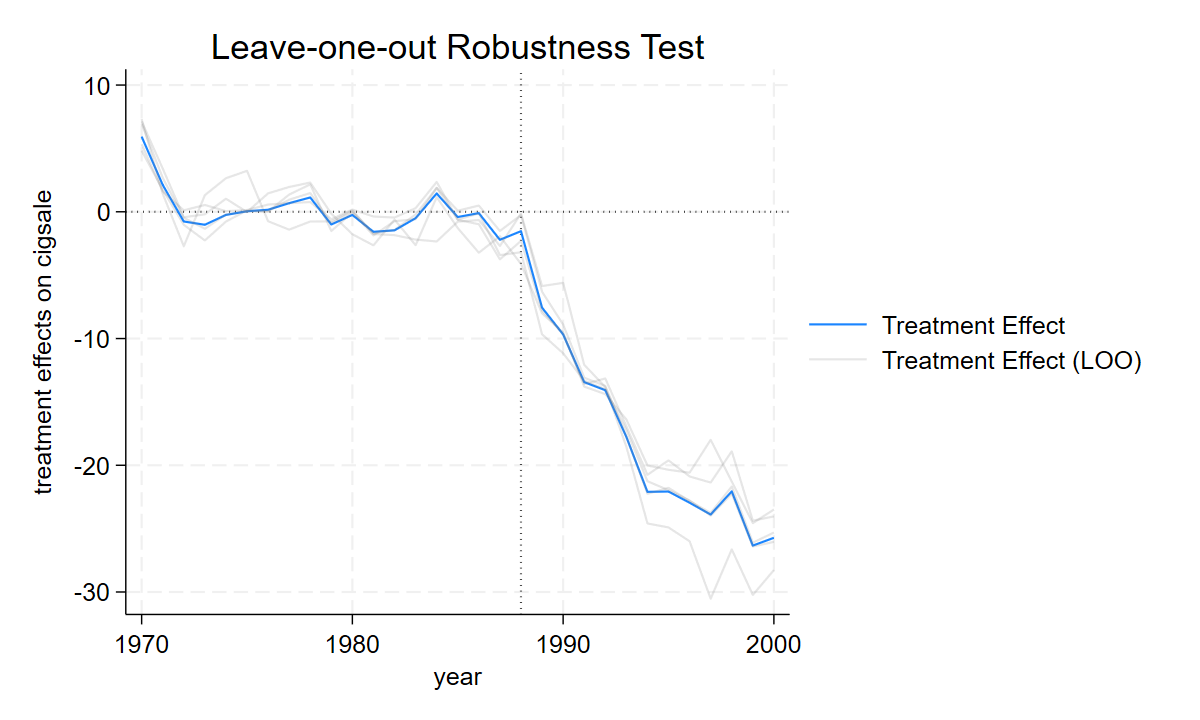
\includegraphics[width=0.66\textwidth]{figures/scm/scm_loo.png}
  \end{center}

  \vspace{-3mm}
  \small
  \textbf{Reading it:} the check of ``Robustness: Leave-One-Out and the
  Predictor Set''. Dropping each of the five weighted donors in turn (gray) barely moves the
  estimated effect (blue). By 2000 the effect is $-25.7$ with a leave-one-out
  range of $[-28.3,\,-23.5]$, so it is not driven by any single state.

\end{frame}

% ── B9: Interpretation ───────────────────────────────────────────────────
\begin{frame}{Interpretation: SCM}

  \begin{columns}[T]
    \begin{column}{0.50\textwidth}
      \textbf{Findings:}
      \begin{itemize}\small
        \item Synthetic California (Utah, Nevada, Montana, Colorado,
          Connecticut) tracks real California closely before 1989.
        \item Gap grows to $\approx 26$ fewer packs by 2000; ATT
          $= -19.0$ over 1989--2000 ($21\,\%$ of the 1988 level of 90
          packs).
        \item In-space placebo $p = 0.026$ (the strong evidence) and
          leave-one-out is stable; the in-time check is weaker (a mild
          pre-1989 drift).
      \end{itemize}
    \end{column}
    \begin{column}{0.46\textwidth}
      \textbf{Caveats:}
      \begin{itemize}\small
        \item SCM gives a trajectory, not a single SE-bearing ATT;
          inference is permutation-based.
        \item Needs a good pre-fit (here RMSPE $1.75$ vs a mean $\sim$116)
          and no spillovers to the donor pool.
      \end{itemize}
      \begin{exampleblock}{\footnotesize Result}
        \footnotesize California's tax cut per-capita consumption by
        $\sim$19 packs/year on average (26 by 2000), a large and robust
        effect (placebo rank 1 of 39).
      \end{exampleblock}
    \end{column}
  \end{columns}

\end{frame}

% ── B-end: when SCM should not be used ───────────────────────────────────
\begin{frame}{When Synthetic Control Should Not Be Used}

  Abadie (2021) sets out the conditions the method needs. Nine ways they
  fail, grouped by what goes wrong.

  \medskip
  \begin{columns}[T]
    \begin{column}{0.48\textwidth}
      \begin{alertblock}{\footnotesize The fit is not there}
        \footnotesize
        \begin{itemize}
          \item Poor pre-treatment fit. Abadie et al.\ (2010) ``recommend
            against'' it,
            and \textbf{a long pre-period cannot rescue a bad fit}.
          \item The treated unit's level is beyond any weighted average of
            donors, and the counterfactual needs the level, not only the
            trend: the estimator ``should not be used in that case''.
          \item Few pre-periods, which invites a fit that is spurious.
        \end{itemize}
      \end{alertblock}
    \end{column}
    \begin{column}{0.48\textwidth}
      \begin{alertblock}{\footnotesize The comparison is not clean}
        \footnotesize
        \begin{itemize}
          \item No uncontaminated donor pool.
          \item Anticipation you cannot date.
          \item Spillovers you can neither drop nor sign.
          \item Several treated units inside the donors' hull: exact fits
            from distant donors hide bias, an ``illusion of perfect fit''.
        \end{itemize}
      \end{alertblock}

      \smallskip
      \begin{block}{\footnotesize The signal is too small}
        \footnotesize
        An effect smaller than the unit's own idiosyncratic volatility, or a
        post-period too short to show it.
      \end{block}
    \end{column}
  \end{columns}

\end{frame}

% ── Section C: SDID Theory ─────────────────────────────────────────────
\section{Synthetic DiD}

% ── C1: From SCM to SDID, in words ───────────────────────────────────────
\begin{frame}{From Synthetic Control to Synthetic DiD}
  \small
  Three ways to say what would have happened to the treated unit:
  \begin{itemize}\small
    \item \textbf{DiD:} it would have changed as the plain average of the
      controls changed. Every control counts the same, every pre-year counts
      the same. Needs parallel trends.
    \item \textbf{Synthetic control:} it would have followed a weighted
      average of donors chosen to reproduce its \emph{level} before $T_0$.
      The effect is the gap after $T_0$.
    \item \textbf{Synthetic DiD} (Arkhangelsky, Athey, Hirshberg, Imbens and
      Wager 2021): a DiD in which the control is a weighted average of donors
      chosen to move \emph{in parallel} with the treated unit before $T_0$,
      and ``before'' is a weighted average of the pre-years that look most
      like the post-period.
  \end{itemize}
  \medskip
  In words: synthetic DiD keeps the DiD comparison, change against change,
  and lets the data choose which controls and which pre-years to compare
  with. The level need not match, only the trend: the level gap is absorbed,
  as in any DiD.
  \medskip
  \begin{block}{\footnotesize Why one of the two sets of weights is enough}
    \footnotesize The bias is the product of two errors: how far the weighted
    donors are from parallel, times how badly the weighted pre-years predict
    the post-period. If either set of weights does its job, the product is
    small.
  \end{block}
\end{frame}

% ── C2: SDID step by step ────────────────────────────────────────────────
\begin{frame}{Synthetic DiD Step by Step}
  \small
  \begin{enumerate}\small
    \item \textbf{Unit weights $\omega_j$}, one per donor, non-negative,
      summing to one: chosen so that the weighted donor average runs parallel
      to the treated unit before $T_0$. An intercept absorbs the level
      difference, so a donor $20$ units higher but moving in step is a good
      donor. A penalty spreads the weight over many donors instead of two or
      three.
    \item \textbf{Time weights $\lambda_t$}, one per pre-year, non-negative,
      summing to one: chosen so that, for the donors, the weighted average of
      the pre-years predicts the post-period average up to a constant.
      Pre-years that look
      like the post-period count; years that look nothing like it get no
      weight.
    \item \textbf{The estimate:} a DiD with those weights.
  \end{enumerate}
  \smallskip
  \begin{center}
    \footnotesize
    \begin{tabular}{@{}lcc@{}}
      \toprule
      & before: $\lambda$-weighted pre-years & after: post-period average \\
      \midrule
      treated unit & $\sum_t \lambda_t\, Y_{1t}$ & $\bar Y_{1,\text{post}}$ \\
      donors, $\omega$-weighted & $\sum_j \omega_j \sum_t \lambda_t\, Y_{jt}$
        & $\sum_j \omega_j\, \bar Y_{j,\text{post}}$ \\
      \bottomrule
    \end{tabular}
  \end{center}
  \smallskip
  $\hat\tau = (\text{after} - \text{before})_{\text{treated}} -
  (\text{after} - \text{before})_{\text{donors}}$: the change of the treated
  unit minus the change of its weighted donors. With every weight equal it is
  the plain DiD; with no intercept, weights that match the level and no
  ``before'' column, it is the synthetic control.
\end{frame}

% ── C2b: What each ingredient buys ───────────────────────────────────────
\begin{frame}{What the Intercept, the Penalty and the Time Weights Do}
  \begin{columns}[T]
    \begin{column}{0.54\textwidth}
      \footnotesize
      \textbf{The intercept.} The weighted donors need only move in parallel
      with the treated unit; the level gap is absorbed. Synthetic control has
      no intercept and must match the level too, which rules out donors that
      are right on trend and off on level.
      \medskip

      \textbf{The penalty on the unit weights.} Its size is a typical
      one-year change of an untreated unit, scaled up by
      $(N_{tr}T_{post})^{1/4}$ (about 1.9 for California). It spreads the weight over more
      donors, so no single one carries the result, and it makes the weights
      unique.
      \medskip

      \textbf{The time weights.} Pre-years that look nothing like the
      post-period get no weight. DiD gives every pre-year the same weight, so
      a distant year in which the donors behaved differently from now pulls
      the counterfactual.
    \end{column}
    \begin{column}{0.44\textwidth}
      \footnotesize
      California, average over 1989--2000, from Arkhangelsky et al.\ (2021):

      \smallskip
      \begin{tabular}{@{}lrr@{}}
        \toprule
        & effect & SE \\
        \midrule
        DiD, uniform weights & $-27.3$ & 17.7 \\
        SC, unit weights & $-19.6$ & 9.9 \\
        SC + intercept & $-11.1$ & 9.5 \\
        SDID, + time weights & $-15.6$ & 8.4 \\
        \bottomrule
      \end{tabular}

      \smallskip
      The intercept moves synthetic control's $-19.6$ to $-11.1$; the time
      weights bring it to $-15.6$. The standard error falls at each step
      (9.9, 9.5, 8.4). When synthetic control and synthetic DiD disagree,
      the paper argues the latter is often more credible.
    \end{column}
  \end{columns}
\end{frame}

% ── C2c: Event-study SDID (Ciccia 2024, sdid_event) ──────────────────────
\begin{frame}{Synthetic DiD Over Time: the Event-Study Version}
  \small
  The single $\hat\tau$ averages the whole post-period. With the same weights
  one can estimate one effect per period since adoption, as in the event
  study of Block 2 (Ciccia 2024):
  \begin{itemize}\small
    \item \textbf{Effects} $\hat\tau_\ell$, $\ell = 1, 2, \dots$: the DiD of
      ``Synthetic DiD Step by Step'' with ``after'' replaced by the $\ell$-th
      period from adoption ($\ell = 1$ is the adoption period). They show whether the effect appears at once,
      builds up or fades.
    \item \textbf{Placebos} $\hat\tau_{-\ell}$, $\ell = 1, 2, \dots$: the same
      DiD with ``after'' replaced by the $\ell$-th period \emph{before}
      adoption, an effect estimated where there was none. Placebos near zero
      say the weighted donors followed the treated unit before adoption; a
      placebo far from zero is a warning about the counterfactual.
  \end{itemize}
  \medskip
  With staggered adoption each cohort has its own weights and its own effects
  by period since adoption; at each $\ell$ the event study averages the
  cohorts, each weighted by its number of treated units. Inference as for the
  single $\hat\tau$: placebo with one treated unit, bootstrap with several.
\end{frame}

% ── C3: Inference, in words ──────────────────────────────────────────────
\begin{frame}{Synthetic DiD Inference, in Words}
  \small
  The estimate is a weighted DiD, so it comes with a standard error. The
  paper gives three ways to get one:
  \begin{itemize}\small
    \item \textbf{Placebo.} Set the treated units aside; give the treatment,
      on paper, to as many controls as there were treated, chosen at random;
      re-estimate; repeat. The spread of the placebo estimates is the
      standard error. The only option with one treated unit, and valid only
      if all units share the same noise variance.
    \item \textbf{Bootstrap.} Resample units with replacement and re-estimate.
      Needs several treated units, so that every resample contains some.
    \item \textbf{Jackknife.} Drop one unit at a time and recompute the
      weighted DiD with the weights held fixed, so SDID runs once. Not
      defined with one treated unit.
  \end{itemize}
  \medskip
  \begin{block}{\footnotesize What to report}
    \footnotesize The method, the seed and the number of replications. The
    point estimate is fixed; the placebo and bootstrap standard errors are
    simulated and move with the draw.
  \end{block}
\end{frame}

% ── C4: SDID vs SCM vs DiD ───────────────────────────────────────────────
\begin{frame}{SDID vs SCM vs DiD: When to Use What}

  \begin{center}
  \small
  \begin{tabular}{p{2.8cm}p{3.2cm}p{3.2cm}p{2.6cm}}
    \toprule
    & \textbf{DiD / TWFE} & \textbf{SCM} & \textbf{SDID} \\
    \midrule
    \# treated units & Many & One (or few) & One or many \\
    Before $T_0$ & Parallel trends \emph{assumed} & Level matched & Trend matched \\
    Unit weights & Uniform & Few donors & More than SCM \\
    Time weights & Uniform & None & Chosen by the data \\
    Standard errors & Cluster SE & Permutation $p$ & Placebo, jackknife,\newline bootstrap \\
    Multiple treated & Yes (C\&S, dCH) & Yes (averages them) & Yes \\
    \bottomrule
  \end{tabular}
  \end{center}

  \medskip
  \textbf{Nesting:} SDID contains both DiD (all weights equal) and SCM (unit
  weights matching the level, no unit fixed effects, no time weights) as
  special cases.

  \smallskip
  \textbf{Staggered adoption:} one block per adoption cohort, each with its
  own weights, then averaged (Clarke, Pailañir, Athey and Imbens 2024).

\end{frame}

% ── Section D: Demo — SDID (California + staggered) ────────────────────
\section{Demo: Synthetic DiD}

% ── D1: Stata code (California) ──────────────────────────────────────────
\begin{frame}[fragile]{Stata: the \texttt{sdid} Command (California)}

\begin{lstlisting}[language=,basicstyle=\ttfamily\footnotesize,
    keywordstyle=\color{MidBlue}\bfseries, commentstyle=\color{gray},
    morekeywords={sdid,gen}, xleftmargin=2mm]
use "$data/smoking.dta", clear
gen treated = (state == 3 & year >= 1989)   // California from 1989

sdid cigsale state year treated, ///
    vce(placebo) seed(1234) reps(100) graph
\end{lstlisting}

  \textbf{Syntax:} \texttt{sdid Y unit time treated [, options]}
  \begin{itemize}\small
    \item \texttt{vce(placebo)}: placebo SEs: the mode for a single
      treated unit (seed + reps pinned for reproducibility).
    \item \texttt{graph}: reweighted control vs treated path, plus the
      $\hat\lambda_t$ time weights.
  \end{itemize}

  \medskip
  \textbf{Result:} ATT $= \mathbf{-15.60}$ packs (SE $8.99$, $p = 0.082$,
  95\% CI $[-33.22,\ 2.01]$), with \texttt{seed(1234) reps(100)}.

  \smallskip
  \footnotesize \alert{Always report both.} The point estimate is stable, the
  placebo SE is not: Clarke et al.\ (2024) get $9.879$ and $p = 0.114$ with a
  different seed and \texttt{reps(50)}, and the original paper reports $8.4$.
  With one treated unit the verdict crosses $p = 0.10$ on the luck of the draw.

\end{frame}

% ── D2: California figure ────────────────────────────────────────────────
\begin{frame}{SDID California: Weighted Trajectories + Time Weights}

  \begin{center}
    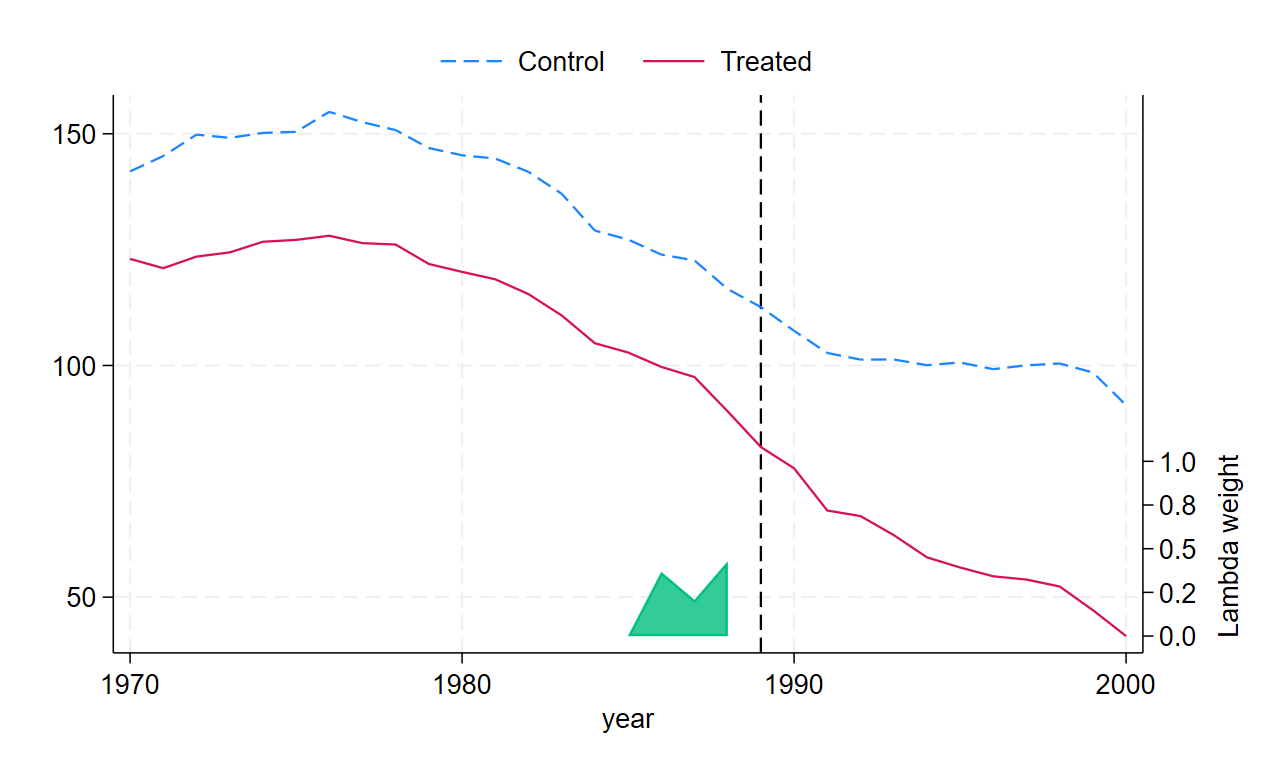
\includegraphics[width=0.56\textwidth]{figures/scm/sdidca_trends1989.png}
  \end{center}

  \vspace{-3mm}
  \small
  \textbf{Reading it:} blue dashed = unit-weighted control average; red =
  California; green = the time weights $\hat\lambda_t$, non-negative and
  summing to one over 1970--1988: $0.37$ on 1986, $0.21$ on 1987, $0.43$ on
  1988, zero on every earlier year. The unit weights $\hat\omega_j$ are
  positive for 28 of the 38 donors (largest $0.12$), where the synthetic control used
  five. One ATT for 1989--2000 is reported; the yearly gaps with their bands
  are the event study two frames on.

\end{frame}

% ── D3: DiD vs SC vs SDID ────────────────────────────────────────────────
\begin{frame}{Same Data, Three Estimators}

  \begin{columns}[T]
    \begin{column}{0.46\textwidth}
      \textbf{California, our \texttt{sdid} output:}
      \smallskip
      \footnotesize
      \begin{tabular}{lc}
        \toprule
        Estimator & ATT (packs) \\
        \midrule
        DiD  & $-27.35$ \\
        SC   & $-19.62$ \\
        \textbf{SDID} & $\mathbf{-15.60}$ \\
        \bottomrule
      \end{tabular}

      \medskip
      \normalsize These reproduce Arkhangelsky et al.\ (2021) exactly
      ($-27.3 / -19.6 / -15.6$).
    \end{column}
    \begin{column}{0.50\textwidth}
      \textbf{Why they differ:}
      \begin{itemize}\small
        \item \textbf{DiD} uses all controls with equal weights, biased
          if pre-trends are not parallel (they are not here).
        \item \textbf{SC} reweights units to match the pre-period level;
          the 2000 gap alone is $\approx -26$.
        \item \textbf{SDID} adds unit \emph{and} time weights (the latter on
          pre-years only) and reports one ATT, the equal-weight average over
          1989--2000 ($-15.6$ vs SC's $-19.6$), with a placebo SE that
          assumes homoskedasticity across states.
      \end{itemize}
    \end{column}
  \end{columns}

\end{frame}

% ── D3b: SDID event study, California (sdid_event) ──────────────────────
\begin{frame}[fragile]{SDID Event Study: California}
  \begin{columns}[T]
    \begin{column}{0.56\textwidth}
      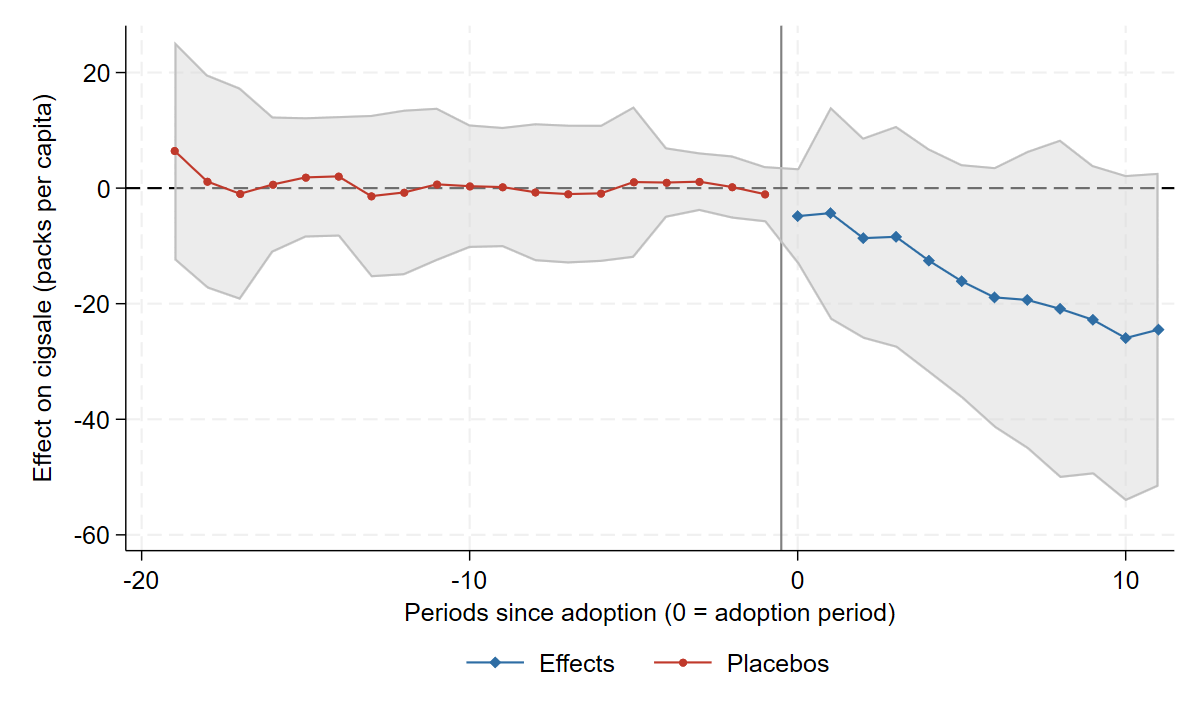
\includegraphics[width=\linewidth]{figures/scm/sdid_event_ca.png}
    \end{column}
    \begin{column}{0.42\textwidth}
      \footnotesize
\begin{lstlisting}[language=,basicstyle=\ttfamily\scriptsize, xleftmargin=0mm]
sdid_event cigsale state year treated, ///
    vce(placebo) brep(100) placebo(all)
\end{lstlisting}
      \texttt{sdid\_event} (Ciccia 2024): ``Synthetic DiD Over Time'' with
      the weights of the \texttt{sdid} run.\\[4pt]
      \textbf{Effects} (blue): $-4.8$ packs in 1989, $-12.5$ in 1993, $-26$
      by 1999. Their average is the ATT of \texttt{sdid}, $-15.6$.\\[4pt]
      \textbf{Placebos} (red): between $-1.4$ and $+2.0$ packs in every pre-year but
      1970 ($+6.5$).\\[4pt]
      \textbf{Bands:} every yearly band includes zero. One treated unit and
      100 placebo draws give standard errors of $4$ to $15$ packs, and the
      ATT's band, $[-33.8,\,2.6]$, includes zero too ($p \approx 0.09$). The
      verdict on California is the permutation rank of the synthetic control,
      first of 39; the event study adds the shape.
    \end{column}
  \end{columns}
\end{frame}

% ── D4: Staggered — Context & Data (gender quotas) ───────────────────────
\begin{frame}{SDID with Staggered Adoption: Context \& Data}

  \begin{columns}[T]
    \begin{column}{0.54\textwidth}
      \textbf{Research question}\\
      Do reserved-seat gender quotas raise women's representation in
      parliament?

      \medskip
      \textbf{Paper / data}\\
      Clarke et al.\ (2024); Bhalotra, Clarke, Gomes \& Venkataramani
      (2023). \texttt{quota\_example.dta}.
      \begin{itemize}\small
        \item \textbf{119 countries}, yearly panel 1990--2015; 9 adopt a
          quota.
        \item Outcome \texttt{womparl} (\% women in parliament);
          treatment \texttt{quota} (0/1).
        \item \textbf{Staggered}: quotas adopted in \textbf{7 different
          years} (2000--2013).
      \end{itemize}
    \end{column}
    \begin{column}{0.42\textwidth}
      \begin{block}{Why SDID here?}
        \footnotesize
        Multiple treated units adopting at different dates. \texttt{sdid}
        handles this by splitting the panel into adoption cohorts (one
        block each) and averaging, so the same engine extends to
        staggered designs.
      \end{block}
    \end{column}
  \end{columns}

\end{frame}

% ── D5: Staggered — command + result + figure ────────────────────────────
\begin{frame}[fragile]{SDID Staggered: Estimation}

  \begin{columns}[T]
    \begin{column}{0.44\textwidth}
\begin{lstlisting}[language=,basicstyle=\ttfamily\scriptsize,
    keywordstyle=\color{MidBlue}\bfseries, commentstyle=\color{gray},
    morekeywords={sdid,use}, xleftmargin=1mm]
use quota_example, clear
sdid womparl country year ///
    quota,                ///
    vce(bootstrap)        ///
    seed(1234) reps(100) graph
\end{lstlisting}

      \footnotesize
      \texttt{vce(bootstrap)}: resamples units (valid with many treated).

      \medskip
      \textbf{Result:} ATT $= \mathbf{+8.03}$ pp\\
      (SE $3.31$, $p = 0.015$, CI $[1.54,\ 14.53]$).\\[3pt]
      Quotas raise women in parliament by $\approx 8$ percentage points.
    \end{column}
    \begin{column}{0.54\textwidth}
      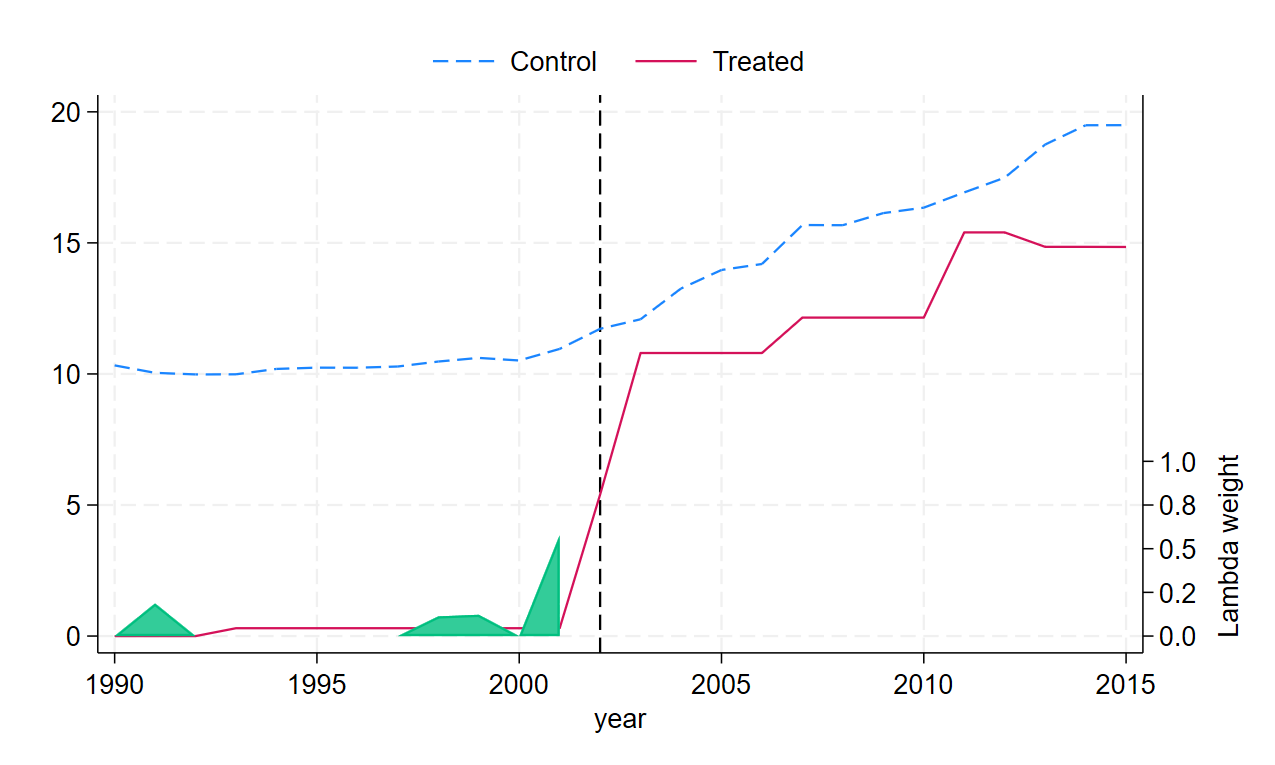
\includegraphics[width=\linewidth]{figures/scm/sdidq_trends2002.png}

      \smallskip\centering\footnotesize
      One adoption cohort (2002): treated countries jump after the quota;
      $\hat\lambda_t$ (green) weight the pre-2002 years.
    \end{column}
  \end{columns}

\end{frame}

% ── D5b: SDID event study, quotas (sdid_event) ──────────────────────────
\begin{frame}[fragile]{SDID Event Study: Quotas, Staggered}
  \begin{columns}[T]
    \begin{column}{0.56\textwidth}
      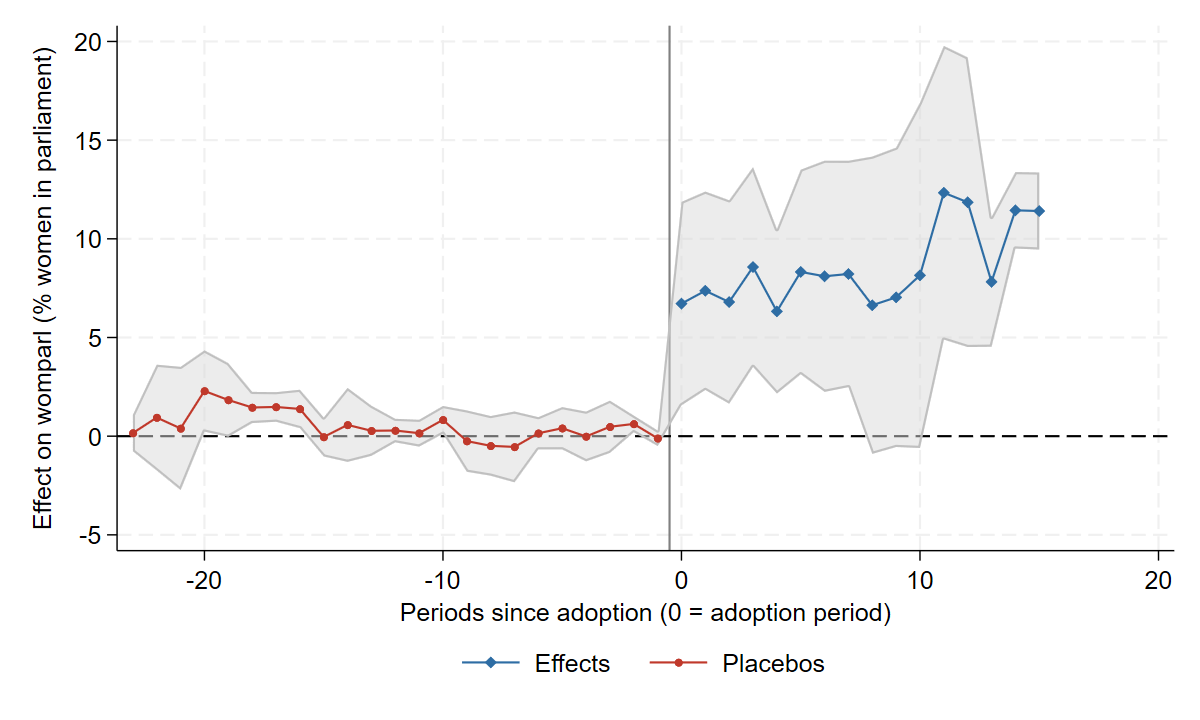
\includegraphics[width=\linewidth]{figures/scm/sdid_event_quota.png}
    \end{column}
    \begin{column}{0.42\textwidth}
      \footnotesize
\begin{lstlisting}[language=,basicstyle=\ttfamily\scriptsize, xleftmargin=0mm]
sdid_event womparl country year quota, ///
    vce(bootstrap) brep(100) placebo(all)
\end{lstlisting}
      One event study across the seven adoption cohorts (nine countries),
      each cohort with its own weights.\\[4pt]
      \textbf{Effects:} $+6.7$ points in the adoption year, $6$ to $9$ over
      the next ten years. Beyond that, $11$ to $12$ ($7.8$ thirteen years
      after adoption), resting on five, three and one countries: the jump is
      a change of composition.\\[4pt]
      \textbf{Placebos:} below one point up to fifteen years before adoption;
      $1.4$ to $2.3$ at 16 to 20 years back (five countries); below one
      again beyond.\\[4pt]
      ATT $= 8.03$, as with \texttt{sdid}; SE $2.49$ here against $3.31$
      there, each from its own bootstrap of 100 replications.
    \end{column}
  \end{columns}
\end{frame}

% ── D4: Takeaways ────────────────────────────────────────────────────────
\begin{frame}{SCM and SDID --- Takeaways}

  \begin{columns}[T]
    \begin{column}{0.48\textwidth}
      \textbf{Synthetic Control Method:}
      \begin{itemize}
        \item Best for 1 treated unit, long pre-period and good pre-fit.
        \item Constructs counterfactual as a convex combination of donors.
        \item Inference via in-space permutation (placebo $p$-values;
          Fisher-exact only under random assignment).
        \item \texttt{synth2} in Stata.
      \end{itemize}
    \end{column}
    \begin{column}{0.48\textwidth}
      \textbf{Synthetic DiD:}
      \begin{itemize}
        \item Adds unit fixed effects and time weights to SC-style unit
          weights.
        \item Unit weights make pre-trends parallel; time weights pick the
          pre-years that predict the post-period.
        \item A single ATT with a standard error, or one effect per period
          since adoption with its placebos.
        \item \texttt{sdid} and \texttt{sdid\_event} in Stata.
      \end{itemize}
    \end{column}
  \end{columns}

  \medskip
  \begin{alertblock}{Decision rule (thumb)}
    \begin{tabular}{ll}
      1 treated unit, trajectory + permutation $p$ & $\to$ SCM \\
      1+ treated units, single ATT + SE       & $\to$ SDID \\
      Staggered adoption                      & $\to$ SDID (cohorts) or C\&S/dCH \\
    \end{tabular}
  \end{alertblock}

\end{frame}

% ── Practical card: SCM and SDID ─────────────────────────────────────────
\begin{frame}{SCM and SDID --- The Practical Answers}

  \begin{columns}[T]
    \begin{column}{0.48\textwidth}
      \textbf{How small a $p$ can I get?}\\
      \footnotesize With 38 donors the permutation test cannot go below
      $1/39 = 0.026$, however large the effect. If a referee wants
      $p < 0.01$, permutation inference cannot give it. And
      \texttt{cutoff()} discards donors, so it moves the $p$ by changing the
      denominator.

      \medskip
      \normalsize\textbf{Which standard error?}\\
      \footnotesize With one treated unit, \texttt{vce(placebo)}; the command
      refuses the bootstrap there. Always report the seed and \texttt{reps()}:
      the point estimate is stable, the placebo SE is not.

      \medskip
      \normalsize\textbf{How long a pre-period?}\\
      \footnotesize Long enough to fit, but length does not rescue a bad fit.
      A poor pre-period fit is a reason not to use the method at all.
    \end{column}
    \begin{column}{0.48\textwidth}
      \begin{block}{\footnotesize What goes in the report}
        \footnotesize
        The path plot with the treated and synthetic series, the weight table so
        the reader can see which donors carry the estimate, the permutation
        $p$-value, and at least one of leave-one-out or the in-time placebo.
        The weights are what makes the exercise auditable by someone who is not
        an econometrician.
      \end{block}

      \smallskip
      \begin{alertblock}{\footnotesize A single ATT can hide everything}
        \footnotesize
        In the staggered quota example the aggregate is $+8.03$ while the seven
        adoption cohorts run from $-3.45$ to $+21.76$. Always look at
        \texttt{e(tau)} before you quote the headline.
      \end{alertblock}
    \end{column}
  \end{columns}

\end{frame}

\end{document}
